\documentclass[12pt,preprint]{aastex}

% has to be before amssymb it seems
\usepackage{color,hyperref}
\definecolor{linkcolor}{rgb}{0,0,0.5}
\hypersetup{colorlinks=true,linkcolor=linkcolor,citecolor=linkcolor,
            filecolor=linkcolor,urlcolor=linkcolor}

\usepackage{url}
\usepackage{algorithmic,algorithm}
\usepackage{amssymb,amsmath}

\usepackage{listings}
\definecolor{lbcolor}{rgb}{0.9,0.9,0.9}
\lstset{language=Python,
        basicstyle=\footnotesize\ttfamily,
        showspaces=false,
        showstringspaces=false,
        tabsize=2,
        breaklines=false,
        breakatwhitespace=true,
        identifierstyle=\ttfamily,
        keywordstyle=\bfseries\color[rgb]{0.133,0.545,0.133},
        commentstyle=\color[rgb]{0.133,0.545,0.133},
        stringstyle=\color[rgb]{0.627,0.126,0.941},
    }

\newcommand{\project}[1]{{\sffamily #1}}
\newcommand{\Python}{\project{Python}}
\newcommand{\numpy}{\project{numpy}}
\newcommand{\bart}{\project{Bart}}
\newcommand{\emcee}{\project{emcee}}
\newcommand{\license}{MIT License}

\newcommand{\paper}{\emph{Article}}

\newcommand{\foreign}[1]{\emph{#1}}
\newcommand{\etal}{\foreign{et\,al.}}
\newcommand{\etc}{\foreign{etc.}}

\newcommand{\Fig}[1]{Figure~\ref{fig:#1}}
\newcommand{\fig}[1]{\Fig{#1}}
\newcommand{\figlabel}[1]{\label{fig:#1}}
\newcommand{\Tab}[1]{Table~\ref{tab:#1}}
\newcommand{\tab}[1]{\Tab{#1}}
\newcommand{\tablabel}[1]{\label{tab:#1}}
\newcommand{\Eq}[1]{Equation~(\ref{eq:#1})}
\newcommand{\eq}[1]{\Eq{#1}}
\newcommand{\eqlabel}[1]{\label{eq:#1}}
\newcommand{\Sect}[1]{Section~\ref{sect:#1}}
\newcommand{\sect}[1]{\Sect{#1}}
\newcommand{\App}[1]{Appendix~\ref{sect:#1}}
\newcommand{\app}[1]{\App{#1}}
\newcommand{\sectlabel}[1]{\label{sect:#1}}
\newcommand{\Algo}[1]{Algorithm~\ref{algo:#1}}
\newcommand{\algo}[1]{\Algo{#1}}
\newcommand{\algolabel}[1]{\label{algo:#1}}

% math symbols
\newcommand{\dd}{\ensuremath{\mathrm{d}}}
\newcommand{\bvec}[1]{\ensuremath{\boldsymbol{#1}}}
\newcommand{\unit}[1]{\ensuremath{\mathrm{#1}}}
\newcommand{\normal}[1]{\ensuremath{\mathcal{N}(#1)}}

\begin{document}

\title{Flexible and rapid exoplanet transit modeling with Bart}

\newcommand{\nyu}{2}
\newcommand{\mpia}{3}
\author{%
    Daniel~Foreman-Mackey\altaffilmark{1,\nyu},
    David~W.~Hogg\altaffilmark{\nyu,\mpia},
    Patrick Cooper\altaffilmark{\nyu}
}
\altaffiltext{1}{To whom correspondence should be addressed:
                        \url{danfm@nyu.edu}}
\altaffiltext{\nyu}{Center for Cosmology and Particle Physics,
                        Department of Physics, New York University,
                        4 Washington Place, New York, NY, 10003, USA}
\altaffiltext{\mpia}{Max-Planck-Institut f\"ur Astronomie,
                        K\"onigstuhl 17, D-69117 Heidelberg, Germany}

\begin{abstract}
With enormous numbers of transiting exoplanets being discovered by
\project{Kepler}, it is finally becoming possible to hierarchically infer the
parameters of the entire population of exoplanets.
A necessary component of these analyses is a tool for high performance
probabilistic transit modeling---sampling the posterior PDF for the
parameters of an arbitrary multi-planet exoplanet system given stellar
light-curve data and parameterized priors.
We present a computationally efficient and extremely flexible system
called \project{Bart} for performing these inferences.
\project{Bart} uses a non-parametric limb-darkening law
for each star; it is much more flexible than the classic analytic
results in current use, at minimal computational cost.
We apply \project{Bart} to all NNN planets observed in the
\project{Kepler} photometric time series for the system Kepler-XXXXX
and the IR light curve of BLAH observed by \project{Spitzer}.
The code is designed so that radial velocity and astrometric observations can
be easily incorporated as further constraints for a joint analysis when
available.

\project{Bart} is implemented in Python and it is available under the
\license\ online at \url{http://dan.iel.fm/bart}.
\end{abstract}

\keywords{%
exoplanets: sickness
---
code: open-source
---
keywords: made-up-by-Hogg
}

\section{Introduction}

The NASA \project{Kepler} mission (DFM CITE) has discovered and
characterized thousands of transiting planets and planet
candidates.
Radial-velocity surveys have discovered hundreds (DFM
CITE), a handful have been directly imaged (DFM CITE, including
Oppenheimer et al), and the ESA \project{Gaia} mission (DFM CITE) is
expected to discover many thousands more astrometrically
Each technique has different sensitivity to exoplanets with different
properties; each technique finds a different subset of the total
exoplanet population; none is complete.
Not even any simple combination of techniques is expected to return a
complete census of exoplanets.

For probabilistic reasoners---``Bayesians'' in some contexts---the
right way to approach these problems is \emph{hierarchical} (DFM CITE
GELMAN OR SOMEONE).
The properties of the overall exoplanet population is parameterized with
``hyperparameters''; at any setting of these hyperparameters, the overall
population plus the modeled selection effects relevant to each observational
program provides the prior probability distribution for the parameters of any
individual observed or observable exoplanet system.
When inference is being performed to obtain the properties of the population
as a whole, the properties of every individual exoplanet are marginalized out,
leaving a marginalized likelihood function or posterior probability
distribution function (posterior PDF) for the population
hyperparameters.
When inference is being performed to obtain the
properties of any individual exoplanetary system, the posterior PDF
for that system is obtained by marginalizing out all \emph{other}
systems and the hyperparameters themselves.
Hierarchical inference
best uses knowledge about \emph{every} observed system to inform
inferences about each \emph{individual} system, and effectively
provides \emph{noise-deconvolved} inferences about the parent
population.
We have implemented a simple hierarchical population
inference previously and demonstrated these properties of hierarchical
inference in this context (DFM CITE HOGG, BOVY, MYERS).

The enormous challenge for this program of hierarchical inference is
that it involves the marginalization out of the parameters of now
thousands of exoplanets in datasets that contain millions to billions
of data point (DFM FIX NUMBERS).
Given the non-triviality of the
relevant noise models and the nonlinearity of exoplanet fitting, this
marginalization is impossible analytically so we must use computationally
expensive approximate methods.
A popular class of algorithm for these sorts
of computations is called Markov chain Monte Carlo (MCMC; DFM CITE).
The computational cost of an accurate Monte Carlo marginalization is very
high but the existence of efficient MCMC algorithms---such as Foreman-Mackey
et al. (DFM)---and optimized likelihood computations makes the prospects for
ambitious hierarchical inference on the ensemble of known exoplanets very
good.

In this \paper, we lay the groundwork for high-performance numerical
marginalization of planetary parameters conditioned on the light curve of
planetary transits.
We recognize that a hierarchical inference
with the set of all known exoplanet data---or even just the
\project{Kepler} set---will require extremely fast and accurate modeling of
exoplanet transit light curves.
In this context, ``modeling'' means sampling the posterior PDF for the
exoplanet parameters given the data and a parameterized prior PDF.
Here we describe and publish high performance open-source code---\bart---for
performing this modeling, and also apply it to real data to demonstrate its
use and value.

In addition to meeting our needs for hierarchical inference, \bart\ is
also flexible in treating stellar limb darkening.
Up to now, most eclipse modeling has made use of extremely useful analytic
approximations \citep{mandel}.
However, these approximations only permit certain kinds of limb-darkening
effects and require the (computationally expensive) evaluation of special
functions.
\bart\ avoids these problems by making use of a non-parametric model for limb
darkening.

\bart\ comprises two main components: a light curve computation engine, and a
model building and fitting  toolkit.
The first component is a standalone Fortran library---with optional Python
bindings---that generates model light curves for very general sets of input
physical parameters.
The second part is a Python module that provides a syntax for modelling and
fitting observed light curves.
This module is built on top of \emcee\ for efficient MCMC sampling of the
posterior probability function for the model paramters conditioned on a
dataset.


\section{How to fit an exoplanet transit}

The procedure for finding the physical parameters of an exoplanetary system
that are consistent with an observed time series is a fairly classic type of
inference problem.
For a given set of physical parameters---including the
planet radii, orbital eccentricities, the observers viewing angle, and other
parameters---we have a ``physical'' description of the data generation
procedure by combining Kepler's equation and some (simplistic) noise model for
the optics and detector.
A generative model like this provides an excellent
likelihood function for the data given those particular parameters.
In this \paper, we will assume that the noise is Gaussian and uncorrelated
(see section SOMESECTION for a discussion of this assumption) so the
observation at a particular time $t_n$ are generated by
\begin{eqnarray}
    f_{\mathrm{obs},n} & = & f_\mathrm{model} (t_n) + \epsilon_n
\end{eqnarray}
where $f_\mathrm{model}$ is a function that includes the effects of geometry
and limb darkening and $\epsilon_n \sim \normal{0, \sigma_n^2}$ is the
stochastic noise model.

Computations of the model $f_\mathrm{model} (t_n)$ involve two parts: the
orbit computation and the effects of stellar limb darkening.
An approximate solution for the orbit can be obtained by solving Kepler's
equation.
This is a standard calculation that we solve in the case of a general
eccentric orbit using Halley's Method.
For the limb darkening, we use a general non-parametric model that is
described in section SOMESECTION.


\subsection{Orbital elements}

In \bart, we parameterize the orbit of a planet with the parameters:
\begin{itemize}
    {\item the mid-transit time $t_0$ of a reference transit,}
    {\item the semi-major axis $a$,}
    {\item the eccentricity $e$,}
    {\item the longitude of perihelion $\varpi$, and}
    {\item the inclination $\bvec{i}$ of the orbital angular momentum unit
           vector with respect to the mean orbital momentum vector of the
           system.}
\end{itemize}
Supplementing these $6\,K$ parameters with the mass of the star $M_\star$ and
the inclination $i_\mathrm{obs}$ of the mean orbital angular momentum vector
with respect to the observer, fully specifies the orbits of the $K$ planets in
a planetary system as a function of time.
Given these parameters and neglecting the planet-planet interactions, we can
solve for the orbit of each planet independently using the standard techniques
\citep[see][for example]{goldstein}.


\subsection{Transit geometry}

The light curve of a transit of a planet in front of a star can be computed by
integrating the amount of stellar light that is occulted by the planet---and
vice-versa---for each position in the orbit.
Assuming that the system is sufficiently distant that we can neglect
three-dimensional effects, the geometry can be specified by three parameters,
the radius of the star $R$, the radius of the planet $p$ and the impact
parameter (in the plane of the sky) $b$.
The geometry of this system (as seen by the observer) is shown in \fig{geom}.
In the plane of the sky, the amount of occulted stellar light can be computed
by the area integral
\begin{eqnarray}\eqlabel{general-occ}
    \lambda (R, p, b) & = & \int_{A_\mathrm{occ}} I(r) \, \dd A
\end{eqnarray}
where $r$ is distance from the center of the star and $A_\mathrm{occ}$ is the
area (in the plane of the sky) where the planet overlaps the star.

For a uniformly illuminated star, $I(r) = 1$ and the occulted fraction of
light is given by
\begin{eqnarray}\eqlabel{uniform-occ}
    \lambda_\mathrm{uniform} (R, p, b) = \left \{ \begin{array}{ll}
            0 & R + p < b \\
            R^2 \, \kappa_1 + p^2 \, \kappa_2 - \kappa_3
                & |R - p| < b \leq R + p \\
            \pi \, p^2 & b \leq R - a \\
            \pi R^2 & b \leq a - R
        \end{array} \right.
\end{eqnarray}
where
\begin{eqnarray}
    \kappa_1 & = & \arccos \left ( \frac{-p^2 + b^2 + R^2}{2 \, b} \right ) \\
    \kappa_2 & = & \arccos \left ( \frac{p^2 + b^2 - R^2}{2\, p \, b}
                           \right ) \\
    \kappa_3 & = & \frac{1}{2} \sqrt{[R + p + b] \, [R - p + b]
                        \, [-R + p + b] \, [R + p - b]} \quad.
\end{eqnarray}
This is similar to Equation (1) from \citet{mandel} but we've explicitly
computed $\lambda_\mathrm{uniform}$ as a function of the stellar radius in
anticipation of the next section.
A derivation of \eq{uniform-occ} can be found online at
\project{MathWorld}\footnote{%
\url{http://mathworld.wolfram.com/Circle-CircleIntersection.html}}.

The impact parameter $b$ in the equations above can be computed from the
physical and observational parameters of the system by solving for the orbit
as described in the previous section and then ``observing'' the system from
infinity.


\subsection{Limb darkening}

In reality, stars are not uniformly bright illuminated on the plane of the
sky.
Instead, they dim towards the edges.
This effect is called \emph{limb darkening}.
\citet{mandel} provide analytic expressions for the
effects of limb darkening for three simple stellar profiles $I(r)$.
Implementations of these results have been ported to most programming
languages and they are used for most---if not all---applications of exoplanet
transit modeling.
Instead of asserting a specific form for the limb darkening
profile (LDP) and relying on these analytic solutions, we use a numerical
approach that can reach high precision with reasonable computational
efficiency---first-order convergence---for \emph{any} LDP.

To achieve this, we approximate the surface of the star as a piecewise
constant function of radius:
\begin{eqnarray}
    I(r) = \left \{ \begin{array}{ll}
        I_0, & 0 \le r < r_0 \\
        I_1, & r_0 \le r < r_1 \\
        \cdots & \\
        I_{N-1}, & r_{N-1} \le r < R \\
        0, & r > R
    \end{array}\right . \quad.
\end{eqnarray}
In this approximation, the integral in \eq{general-occ} simplifies to the sum
\begin{eqnarray}\eqlabel{numerical-occ}
    \lambda_\mathrm{numer} (R, p, b) & = & \sum_{n=1}^N w_n (p, b) \, I_n \\
                                     & = & \bvec{w} (p, b) \cdot \bvec{I}
\end{eqnarray}
where $w_n(a, b)$ encapsulates all the geometry.
The specific form of $w_n$
can be computed using \eq{uniform-occ}
\begin{eqnarray}
    w_n (p, b) & = & \lambda_\mathrm{uniform} (r_{n}, p, b)
                   - \lambda_\mathrm{uniform} (r_{n-1}, p, b)
\end{eqnarray}
if we define $r_{-1} \equiv 0$ and $r_N \equiv R$.

The light curve produced by \eq{numerical-occ} is very general because there is
no constraint on the positions of the bin edges $r_n$ or on the intensity
levels $I_n$.
It is also a good idea to use this method for several reasons:
\begin{enumerate}
    {\item a reason}
    {\item another reason}
\end{enumerate}

One remaining issue with \eq{numerical-occ} is the question of normalization.
There is currently an infinite degeneracy between the overall normalization of
the LDP and the flux of the star itself.
To break this degeneracy, we add one constraint on the intensity values.
Namely, the surface integral of $I(r)$
should be equal to one
\begin{eqnarray}
    \sum_{n=1}^{N} I_n \, \left [ r_n^2 - r_{n-1}^2 \right ]
    & \equiv & \frac{1}{\pi} \quad.
\end{eqnarray}


\section{Kepler KOI XXX}

\section{GALEX JXXX-XXX}

\section{Discussion}

What is so good about what we have done?

What are the limitations of what we have done?

We didn't do anything beyond limb darkening:  No sunspots or convection.
How could we (in principle) make those changes within the \bart\ framework?

Related to the above, are there elliptical generalizations of any of the above?

We didn't do anything about reflection or emission from the companion.
How could we (in principle) make that change within the framework?
Along these lines, \bart\ could be used to model eclipsing binaries,
in which both members of the binary have non-trivial limb darkening.

Please use our code.  It is available at XXX.

\acknowledgments


\newcommand{\arxiv}[1]{\href{http://arxiv.org/abs/#1}{arXiv:#1}}
\begin{thebibliography}{}\raggedright

\bibitem[Goldstein et al.(2002)]{goldstein}
    Goldstein, H., Poole, C., \& Safko, J.\ 2002, \emph{Classical mechanics}
    (3rd ed.), Addison-Wesley

\bibitem[Mandel \& Agol(2002)]{mandel}
        Mandel, K., \& Agol, E.\ 2002, \apjl, 580, L171
        \arxiv{astro-ph/0210099}

\end{thebibliography}


\clearpage

\begin{deluxetable}{c ccc}

% \tabletypesize{\small}
\tablecolumns{4}
\tablewidth{0pc}

\tablecaption{  }

\tablehead{
    \colhead{} & \colhead{$X_{[0.16]}$}
               & \colhead{$X_{[0.5]}$}
               & \colhead{$X_{[0.84]}$}}

\startdata

$P\,[\mathrm{days}]$ & 3.234690 & 3.234714 & 3.234738 \\
$a/R_\star$ & 7.049953 & 7.049987 & 7.050021 \\
$r/R_\star$ & 0.09538 & 0.09554 & 0.09570 \\
$t_0\,[\mathrm{days}]$ & 1.7998 & 1.8011 & 1.8024 \\
$i\,[\mathrm{deg}]$ & 86.930 & 86.961 & 86.993 \\


\enddata


\end{deluxetable}


\begin{figure}[htbp]
    \begin{center}
        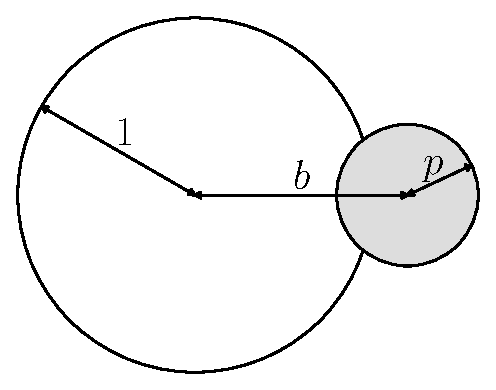
\includegraphics[width=\textwidth]{figures/geom.pdf}
    \end{center}
    \caption{The geometry of a single point in a transit light curve when a
        planet of radius $p$ transits in front of a star of radius $R$. The
        instantaneous impact parameter $b$ is the projected distance between
        the center of the star and the center of the planet on the sky. The
        gray annuli show the bins for the model of the limb darkening of the
        star. \figlabel{geom}}
\end{figure}

\begin{figure}[htbp]
    \begin{center}
        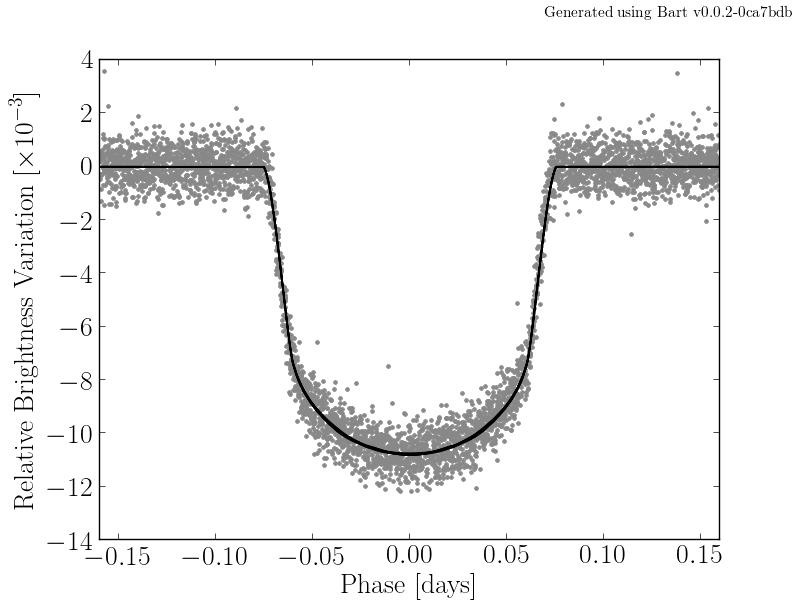
\includegraphics[width=\textwidth]{figures/k6-lc.png}
    \end{center}
    \caption{The observed light curve for Kepler-6b folded on the median
        of posterior period of HOWMANY days. The data are shown as gray points
        and the HOWMANY samples from the posterior fit are shown as black
        lines. \figlabel{k6-lc}}
\end{figure}

\begin{figure}[htbp]
    \begin{center}
        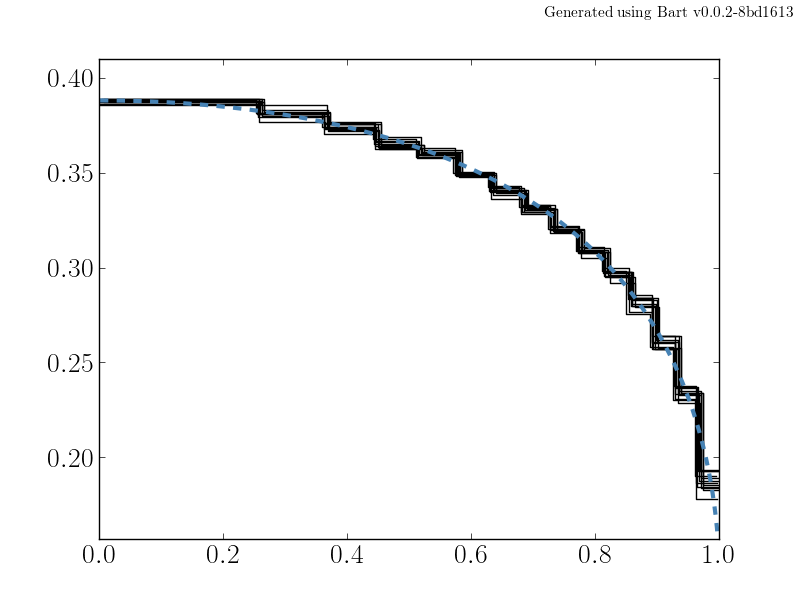
\includegraphics[width=\textwidth]{figures/k6-ldp.png}
    \end{center}
    \caption{Samples from the posterior PDF for the limb darkening profile for
        Kepler-6. The standard Kepler profile (CITE) is given by the blue
        dashed line. \figlabel{k6-ldp}}
\end{figure}

\begin{figure}[htbp]
    \begin{center}
        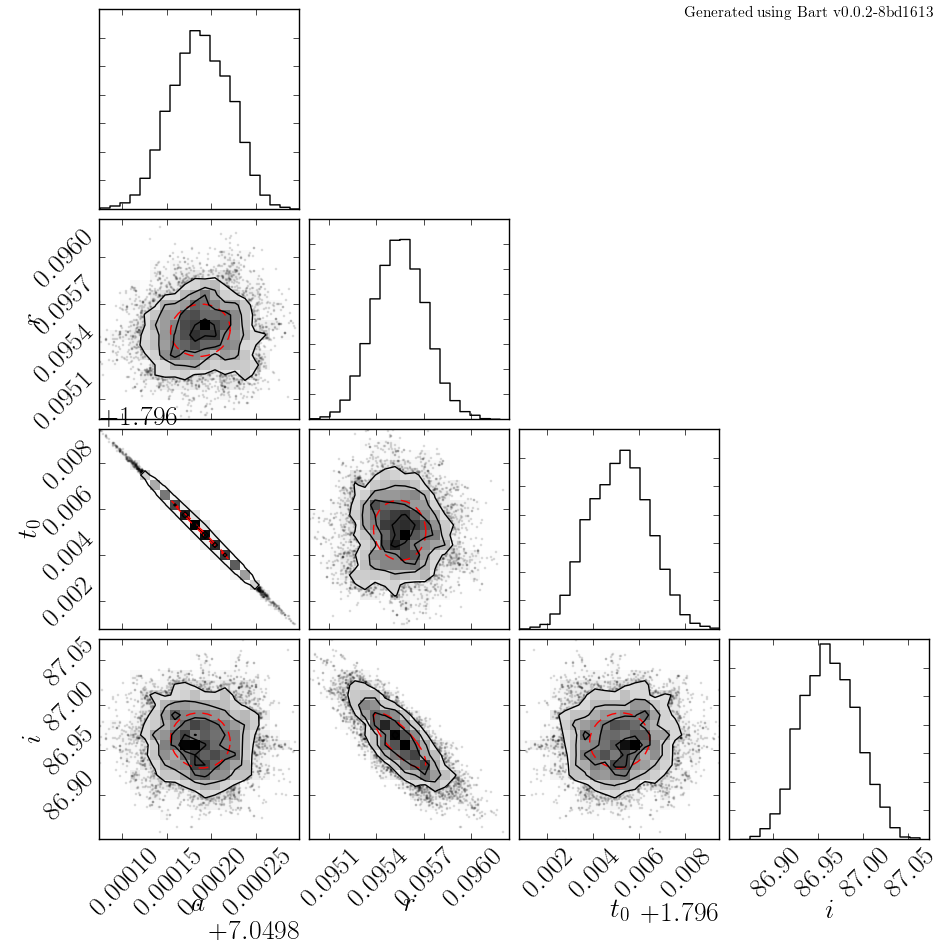
\includegraphics[width=\textwidth]{figures/k6-corner.png}
    \end{center}
    \caption{The marginalized posterior distributions over the fit parameters.
        Each of the one-dimensional histograms show the fully marginalized
        distribution for a single parameter. The two-dimensional contour plots
        show the covariances between the parameters. On the contour plots, the
        levels show the 0.5-, 1-, 1.5- and 2-$\sigma$ levels and the points
        are samples drawn directly from the MCMC. \figlabel{k6-corner}}
\end{figure}


\end{document}
